%% SECTION HEADER /////////////////////////////////////////////////////////////////////////////////////
\section{FCN pixel-wise segmentation models}
\label{sec52}

%% SECTION CONTENT ////////////////////////////////////////////////////////////////////////////////////

%% SUBSECTION HEADER //////////////////////////////////////////////////////////////////////////////////
\subsection{Numerical cases}
\label{sec521}

\begin{figure} [!h]
	\centering
	\begin{subfigure}[b]{.48\textwidth}
		\centering
		\includegraphics[width=.9\textwidth]{Figures/Chapter_5/RMS_flat_shell_Vz_448_500x500bottom.png}
		\caption{}
		\label{fig:RMS_bottom_448}
	\end{subfigure}
	\hfill
	\begin{subfigure}[b]{.48\textwidth}
		\centering
		\includegraphics[width=.9\textwidth]{Figures/Chapter_5/UNet_num_269.png}
		\caption{Res-UNet}
		\label{fig:unet_269}	
	\end{subfigure}
	\hfill
	\begin{subfigure}[b]{.48\textwidth}
		\centering
		\includegraphics[width=0.9\textwidth]{Figures/Chapter_5/VGG16_autoencoder_269.png}
		\caption{VGG16 encoder-decoder}
		\label{fig:vgg16_269}
	\end{subfigure}
	\hfill
	\begin{subfigure}[b]{.48\textwidth}
		\centering
		\includegraphics[width=0.9\textwidth]{Figures/Chapter_5/PSPNet_269.png}
		\caption{PSPNet}
		\label{fig:pspnet_269}	
	\end{subfigure}
	\hfill
	\begin{subfigure}[b]{.48\textwidth}
		\centering
		\includegraphics[width=0.9\textwidth]{Figures/Chapter_5/FCN_DenseNet_269.png}
		\caption{FCN-DenseNet}
		\label{fig:densenet_269}
	\end{subfigure}
	\hfill
	\begin{subfigure}[b]{.48\textwidth}
		\centering
		\includegraphics[width=0.9\textwidth]{Figures/Chapter_5/GCN_269.png}
		\caption{GCN}
		\label{fig:gcn_269}	
	\end{subfigure}
	\caption{First delamination case based on numerical data.}
	\label{fig:rms_first_case}
\end{figure}

%%%%%%%%%%%%%%%%%%%%%%%%%%%%%%%%%%%%%%%%%%%%%%%%%%%%%%%%%%%%%%%%%%%%%%%%%%%%%%%%

\begin{figure} [!h]
	\centering
	\begin{subfigure}[b]{.48\textwidth}
		\centering
		\includegraphics[width=0.9\textwidth]{Figures/Chapter_5/RMS_flat_shell_Vz_456_500x500bottom.png}
		\caption{}
		\label{fig:RMS_bottom_456}
	\end{subfigure}
	\hfill
	\begin{subfigure}[b]{.48\textwidth}
		\centering
		\includegraphics[width=0.9\textwidth]{Figures/Chapter_5/UNet_num_301.png}
		\caption{Res-UNet}
		\label{fig:unet_301}	
	\end{subfigure}
	\hfill
	\begin{subfigure}[b]{.48\textwidth}
		\centering
		\includegraphics[width=0.9\textwidth]{Figures/Chapter_5/VGG16_autoencoder_301.png}
		\caption{VGG16 encoder-decoder}
		\label{fig:vgg16_301}
	\end{subfigure}
	\hfill
	\begin{subfigure}[b]{.48\textwidth}
		\centering
		\includegraphics[width=0.9\textwidth]{Figures/Chapter_5/PSPNet_301.png}
		\caption{PSPNet}
		\label{fig:pspnet_301}	
	\end{subfigure}
	\hfill
	\begin{subfigure}[b]{.48\textwidth}
		\centering
		\includegraphics[width=0.9\textwidth]{Figures/Chapter_5/FCN_DenseNet_301.png}
		\caption{FCN-DenseNet}
		\label{fig:densenet_301}
	\end{subfigure}
	\hfill
	\begin{subfigure}[b]{.48\textwidth}
		\centering
		\includegraphics[width=0.9\textwidth]{Figures/Chapter_5/GCN_301.png}
		\caption{GCN}
		\label{fig:gcn_301}	
	\end{subfigure}
	\caption{Second delamination case based on numerical data.}
	\label{fig:rms_second_case}
\end{figure}

%%%%%%%%%%%%%%%%%%%%%%%%%%%%%%%%%%%%%%%%%%%%%%%%%%%%%%%%%%%%%%%%%%%%%%%%%%%%%%%%

\begin{figure} [!h]
	\centering
	\begin{subfigure}[b]{.48\textwidth}
		\centering
		\includegraphics[width=0.9\textwidth]{Figures/Chapter_5/RMS_flat_shell_Vz_438_500x500bottom.png}
		\caption{}
		\label{fig:RMS_bottom_438}
	\end{subfigure}
	\hfill
	\begin{subfigure}[b]{.48\textwidth}
		\centering
		\includegraphics[width=0.9\textwidth]{Figures/Chapter_5/UNet_num_229.png}
		\caption{Res-UNet}
		\label{fig:unet_229}	
	\end{subfigure}
	\hfill
	\begin{subfigure}[b]{.48\textwidth}
		\centering
		\includegraphics[width=0.9\textwidth]{Figures/Chapter_5/VGG16_autoencoder_229.png}
		\caption{VGG16 encoder-decoder}
		\label{fig:vgg16_229}
	\end{subfigure}
	\hfill
	\begin{subfigure}[b]{.48\textwidth}
		\centering
		\includegraphics[width=0.9\textwidth]{Figures/Chapter_5/PSPNet_229.png}
		\caption{PSPNet}
		\label{fig:pspnet_229}	
	\end{subfigure}
	\hfill
	\begin{subfigure}[b]{.48\textwidth}
		\centering
		\includegraphics[width=0.9\textwidth]{Figures/Chapter_5/FCN_DenseNet_229.png}
		\caption{FCN-DenseNet}
		\label{fig:densenet_229}
	\end{subfigure}
	\hfill
	\begin{subfigure}[b]{.48\textwidth}
		\centering
		\includegraphics[width=0.9\textwidth]{Figures/Chapter_5/GCN_229.png}
		\caption{GCN}
		\label{fig:gcn_229}	
	\end{subfigure}
	\caption{Third delamination case based on numerical data.}
	\label{fig:rms_third_case}
\end{figure}

%%%%%%%%%%%%%%%%%%%%%%%%%%%%%%%%%%%%%%%%%%%%%%%%%%%%%%%%%%%%%%%%%%%%%%%%%%%%%%%%

\begin{figure} [!h]
	\centering
	\begin{subfigure}[b]{.48\textwidth}
		\centering
		\includegraphics[width=0.9\textwidth]{Figures/Chapter_5/RMS_flat_shell_Vz_397_500x500bottom.png}
		\caption{}
		\label{fig:RMS_bottom_397}
	\end{subfigure}
	\hfill
	\begin{subfigure}[b]{.48\textwidth}
		\centering
		\includegraphics[width=0.9\textwidth]{Figures/Chapter_5/UNet_num_65.png}
		\caption{Res-UNet}
		\label{fig:unet_65}	
	\end{subfigure}
	\hfill
	\begin{subfigure}[b]{.48\textwidth}
		\centering
		\includegraphics[width=0.9\textwidth]{Figures/Chapter_5/VGG16_autoencoder_65.png}
		\caption{VGG16 encoder-decoder}
		\label{fig:vgg16_65}
	\end{subfigure}
	\hfill
	\begin{subfigure}[b]{.48\textwidth}
		\centering
		\includegraphics[width=0.9\textwidth]{Figures/Chapter_5/PSPNet_65.png}
		\caption{PSPNet}
		\label{fig:pspnet_65}	
	\end{subfigure}
	\hfill
	\begin{subfigure}[b]{.48\textwidth}
		\centering
		\includegraphics[width=0.9\textwidth]{Figures/Chapter_5/FCN_DenseNet_65.png}
		\caption{FCN-DenseNet}
		\label{fig:densenet_65}
	\end{subfigure}
	\hfill
	\begin{subfigure}[b]{.48\textwidth}
		\centering
		\includegraphics[width=0.9\textwidth]{Figures/Chapter_5/GCN_65.png}
		\caption{GCN}
		\label{fig:gcn_65}	
	\end{subfigure}
	\caption{Fourth delamination case based on numerical data.}
	\label{fig:rms_fourth_case}
\end{figure}
\clearpage

%%%%%%%%%%%%%%%%%%%%%%%%%%%%%%%%%%%%%%%%%%%%%%%%%%%%%%%%%%%%%%%%%%%%%%%%%%%%%%%%%
%\begin{table}[ht!]
%	\centering
%	\caption{\(IoU\) of Numerical cases}
%	\label{tab:table_numerical_cases}
%	{
%		\begin{tabular}{lcccc}
%			\toprule
%			Model & 1st case & 2nd case & 3rd case & 4th case \\ 
%			\midrule 
%			Res-UNet & \(0.50\) & \(0.45\) & \(0.67\) & \(0.80\) \\ 
%			VGG16 encoder-decoder & \(0.51\) & \(0.69\) & \(0.75\) & \(0.65\)\\ 
%			PSPNet & \(0.39\) & \(0.00\) & \(0.44\)  & \(0.77\) \\ 
%			FCN-DenseNet & \(0.73\) & \(0.52\) & \(0.66\) & \(0.72\) \\
%			GCN & \(0.79\) & \(0.71\) & \(0.72\) & \(0.86\) \\ 
%			\bottomrule
%		\end{tabular}
%	}
%\end{table}
%%%%%%%%%%%%%%%%%%%%%%%%%%%%%%%%%%%%%%%%%%%%%%%%%%%%%%%%%%%%%%%%%%%%%%%%%%%%%%%%
%%%%%%%%%%%%%%%%%%%%%%%%%%%%%%%%%%%%%%%%%%%%%%%%%%%%%%%%%%%%%%%%%%%%%%%%%%%%%%%%
\begin{table}[ht!]
	\centering
	\caption{Evaluation metrics of the four numerical cases}
	\begin{tabular}{cccccc}
		\toprule
		\multirow{2}{*}{Model} & \multirow{2}{*}{case number} & \multicolumn{1}{c}{\multirow{2}{*}{A [mm\textsuperscript{2}]}} & \multicolumn{3}{c}{Predicted output} \\ 
		\cmidrule(lr){4-6} & & & \multicolumn{1}{c}{IoU} & \multicolumn{1}{c}{\(\hat{A}\) [mm\textsuperscript{2}]} & \(\epsilon\) \\
		\midrule
		\multirow{4}{*}{Res-UNet} 
		& 1 & 717 & \multicolumn{1}{c}{0.50} & \multicolumn{1}{c}{402} & \(43.93\%\) \\ 
		& 2 & 257 & \multicolumn{1}{c}{0.45} & \multicolumn{1}{c}{143} & \(44.36\%\) \\ 
		& 3 & 105 & \multicolumn{1}{c}{0.67} & \multicolumn{1}{c}{88} & \(16.19\%\) \\ 
		& 4 & 537 & \multicolumn{1}{c}{0.80} & \multicolumn{1}{c}{478} & \(10.99\%\) \\ 
		\midrule
		\multirow{4}{*}{VGG16 encoder-decoder} 
		& 1 & 717 & \multicolumn{1}{c}{0.51} & \multicolumn{1}{c}{410} & \(42.82\%\) \\ 
		& 2 & 257 & \multicolumn{1}{c}{0.69} & \multicolumn{1}{c}{203} & \(21.01\%\) \\ 
		& 3 & 105 & \multicolumn{1}{c}{0.75} & \multicolumn{1}{c}{117} & \(11.43\%\) \\ 
		& 4 & 537 & \multicolumn{1}{c}{0.65} & \multicolumn{1}{c}{385} & \(28.31\%\) \\ 
		\midrule
		\multirow{4}{*}{FCN-DenseNet} 
		& 1 & 717 & \multicolumn{1}{c}{0.73} & \multicolumn{1}{c}{1073} & \(49.65\%\) \\ 
		& 2 & 257 & \multicolumn{1}{c}{0.52} & \multicolumn{1}{c}{505} & \(96.50\%\) \\ 
		& 3 & 105 & \multicolumn{1}{c}{0.66} & \multicolumn{1}{c}{118} & \(12.38\%\) \\ 
		& 4 & 537 & \multicolumn{1}{c}{0.72} & \multicolumn{1}{c}{815} & \(51.77\%\) \\ 
		\midrule
		\multirow{4}{*}{PSPNet} 
		& 1 & 717 & \multicolumn{1}{c}{0.39} & \multicolumn{1}{c}{596} & \(16.88\%\) \\ 
		& 2 & 257 & \multicolumn{1}{c}{0.00} & \multicolumn{1}{c}{0} & \(-\%\) \\ 
		& 3 & 105 & \multicolumn{1}{c}{0.44} & \multicolumn{1}{c}{156} & \(48.57\%\) \\ 
		& 4 & 537 & \multicolumn{1}{c}{0.77} & \multicolumn{1}{c}{610} & \(13.59\%\) \\ 
		\midrule
		\multirow{4}{*}{GCN} 
		& 1 & 717 & \multicolumn{1}{c}{0.79} & \multicolumn{1}{c}{666} & \(7.11\%\) \\ 
		& 2 & 257 & \multicolumn{1}{c}{0.71} & \multicolumn{1}{c}{215} & \(16.34\%\) \\ 
		& 3 & 105 & \multicolumn{1}{c}{0.72} & \multicolumn{1}{c}{177} & \(68.57\%\) \\ 
		& 4 & 537 & \multicolumn{1}{c}{0.86} & \multicolumn{1}{c}{523} & \(2.61\%\) \\ 
		\bottomrule
	\end{tabular}	
	\label{tab:RMS_num_cases}
\end{table}
%%%%%%%%%%%%%%%%%%%%%%%%%%%%%%%%%%%%%%%%%%%%%%%%%%%%%%%%%%%%%%%%%%%%%%%%%%%%%%%%
%%%%%%%%%%%%%%%%%%%%%%%%%%%%%%%%%%%%%%%%%%%%%%%%%%%%%%%%%%%%%%%%%%%%%%%%%%%%%%%%
\begin{table}[ht!]
	\centering
	\caption{Analysis of numerical cases}
	\label{tab:table_all_numerical_cases}
	{
		\begin{tabular}{lcc}
			\toprule
			Model & mean \(IoU\) & max \(IoU\) \\ 
			\midrule 
			Res-UNet & \(0.66\) & \(0.89\) \\ 
			VGG16 encoder-decoder & \(0.57\) & \(0.84\) \\ 
			FCN-DenseNet & \(0.68\) & \(0.92\) \\ 
			PSPNet & \(0.55\) & \(0.91\) \\ 
			GCN & \(0.76\) & \(0.93\) \\ 
			\bottomrule
		\end{tabular}
	}
\end{table}
%%%%%%%%%%%%%%%%%%%%%%%%%%%%%%%%%%%%%%%%%%%%%%%%%%%%%%%%%%%%%%%%%%%%%%%%%%%%%%%%
%%%%%%%%%%%%%%%%%%%%%%%%%%%%%%%%%%%%%%%%%%%%%%%%%%%%%%%%%%%%%%%%%%%%%%%%%%%%%%%%
\begin{table}[ht!]
	\centering
	\caption{Model parameters}
	\label{tab:table_parameters}
	{
		\begin{tabular}{lc}
			\toprule
			Model & Total parameters ($\approx$) \\ 
			\midrule 
			Res-UNet & \(52\times 10^{6}\) \\ 
			VGG16 encoder-decoder & \(37.3\times 10^{6}\) \\ 
			FCN-DenseNet & \(2.5\times 10^{6}\) \\ 
			PSPNet & \(6.6\times 10^{6}\) \\ 
			GCN & \(36\times 10^{6}\) \\ 
			\bottomrule
		\end{tabular}
	}
\end{table}
\clearpage
%%%%%%%%%%%%%%%%%%%%%%%%%%%%%%%%%%%%%%%%%%%%%%%%%%%%%%%%%%%%%%%%%%%%%%%%%%%%%%%%
\subsection{Experimental cases}
\label{sec522}
%%%%%%%%%%%%%%%%%%%%%%%%%%%%%%%%%%%%%%%%%%%%%%%%%%%%%%%%%%%%%%%%%%%%%%%%%%%%%%%%
\begin{figure} [!h]
	\centering
	\begin{subfigure}[b]{.48\textwidth}
		\centering
		\includegraphics[width=0.9\textwidth]{Figures/Chapter_5/ERMS_with_label.png}
		\caption{}
		\label{fig:ERMS_with_label}
	\end{subfigure}
	\hfill
	\begin{subfigure}[b]{.48\textwidth}
		\centering
		\includegraphics[width=0.9\textwidth]{Figures/Chapter_5/Fig_UNET_7.png}
		\caption{Res-UNet}
		\label{fig:unet_exp_erms}	
	\end{subfigure}
	\hfill
	\begin{subfigure}[b]{.48\textwidth}
		\centering
		\includegraphics[width=0.9\textwidth]{Figures/Chapter_5/Fig_VGG16_7.png}
		\caption{VGG16 encoder-decoder}
		\label{fig:vgg16_exp_erms}
	\end{subfigure}
	\hfill
	\begin{subfigure}[b]{.48\textwidth}
		\centering
		\includegraphics[width=0.9\textwidth]{Figures/Chapter_5/Fig_PSPNET_7.png}
		\caption{PSPNet}
		\label{fig:pspnet_exp_erms}	
	\end{subfigure}
	\hfill
	\begin{subfigure}[b]{.48\textwidth}
		\centering
		\includegraphics[width=0.9\textwidth]{Figures/Chapter_5/Fig_FCN_DenseNet_7.png}
		\caption{FCN-DenseNet}
		\label{fig:densenet_exp_erms}
	\end{subfigure}
	\hfill
	\begin{subfigure}[b]{.48\textwidth}
		\centering
		\includegraphics[width=0.9\textwidth]{Figures/Chapter_5/Fig_GCN_7.png}
		\caption{GCN}
		\label{fig:gcn_exp_erms}	
	\end{subfigure}
	\caption{Fourth delamination case based on numerical data.}
	\label{fig:exp_erms__case}
\end{figure}
\clearpage

